%
% dreieck.tex -- Dreiecksfunktion
%
% (c) 2018 Prof Dr Andreas Müller, Hochschule Rapperswil
%
\documentclass[tikz]{standalone}
\usepackage{times}
\usepackage{amsmath}
\usepackage{txfonts}
\usepackage[utf8]{inputenc}
\usepackage{graphics}
\usepackage{color}
\usetikzlibrary{arrows,intersections}
\usepackage{pgfplots}
\begin{document}
\definecolor{darkgreen}{rgb}{0,0.6,0}
\input{triangle.tex}
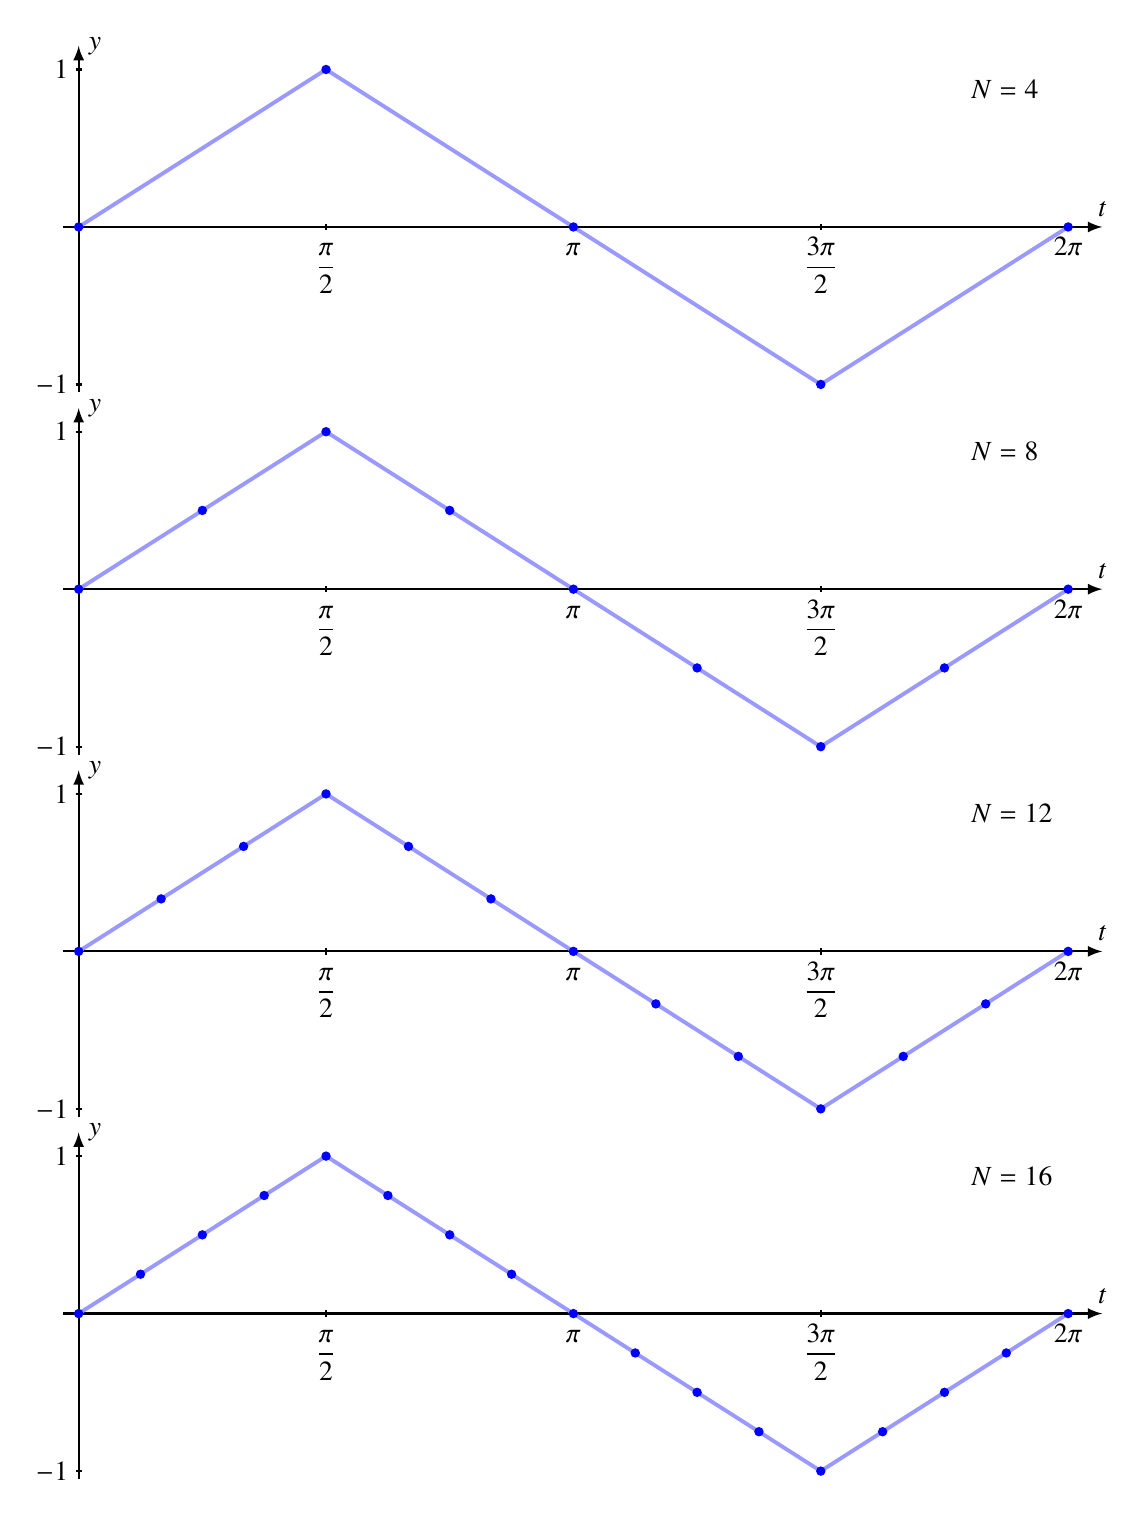
\begin{tikzpicture}[>=latex,thick,scale=2]

\def\pizahl{3.14159}

\def\raster#1#2{
\draw[->] (-0.1,0)--(6.5,0) coordinate[label=$t$];
\draw[->] (0,-1.05)--(0,1.15) coordinate[label={right:$y$}];

\draw ({1*\pizahl/2},-0.02)--({1*\pizahl/2},0.02);
\node at ({1*\pizahl/2},0) [below] {$\displaystyle\frac{\mathstrut\pi}2$};
\draw ({2*\pizahl/2},-0.02)--({2*\pizahl/2},0.02);
\node at ({2*\pizahl/2},0) [below] {$\displaystyle\mathstrut\pi$};
\draw ({3*\pizahl/2},-0.02)--({3*\pizahl/2},0.02);
\node at ({3*\pizahl/2},0) [below] {$\displaystyle\frac{3\mathstrut\pi}2$};
\draw ({4*\pizahl/2},-0.02)--({4*\pizahl/2},0.02);
\node at ({4*\pizahl/2},0) [below] {$\displaystyle2\mathstrut\pi$};

\draw (-0.02,1)--(0.02,1);
\node at (0,1) [left] {$1$};
\draw (-0.02,-1)--(0.02,-1);
\node at (0,-1) [left] {$-1$};

\draw[color=blue!40,line width=1.4pt] (0,0)--({\pizahl/2},1)--({\pizahl},0)--({1.5*\pizahl},-1)--({2*\pizahl},0);

\csname#2\endcsname

\fill[color=blue] (0,0) circle[radius=0.03];
\foreach \x in {1,...,#1}{
	\pgfmathparse{\x*\pizahl/(2*#1)}
	\xdef\argument{\pgfmathresult}
	\fill[color=blue] ({\argument},{\x/#1})
		circle[radius=0.03];
	\fill[color=blue] ({0.5*\pizahl+\argument},{1-\x/#1})
		circle[radius=0.03];
	\fill[color=blue] ({1.0*\pizahl+\argument},{-\x/#1})
		circle[radius=0.03];
	\fill[color=blue] ({1.5*\pizahl+\argument},{-1+\x/#1})
		circle[radius=0.03];
}

\pgfmathparse{4*#1}
\xdef\N{\pgfmathresult}

\pgfplotsset{
/pgf/number format/textnumber/.style={fixed zerofill,precision=0}
}

\node at (5.6,1.0) [below right] {$N=\pgfmathprintnumber[textnumber]{\N}$};

}

\raster{1}{eins}

\begin{scope}[yshift = -2.3cm]
\raster{2}{zwei}
\end{scope}

\begin{scope}[yshift = -4.6cm]
\raster{3}{drei}
\end{scope}

\begin{scope}[yshift = -6.9cm]
\raster{4}{vier}
\end{scope}

%\begin{scope}[yshift = -9.2cm]
%\raster{10}{zehn}
%\end{scope}

\end{tikzpicture}
\end{document}
